\documentclass[supercite]{HustGraduPaper}
%进行个人信息设置
\title{生物信息学上机实验} %论文题目
\author{张皓鸿} %作者姓名
\date{\today} %日期,默认当日
\school{生命科学与技术学院} %院系名称
\classnum{登峰1901班} %专业班级
\stunum {U201912537} %学号

%添加自己要用的其他宏包
\usepackage{xltxtra}
\usepackage{bm}
\usepackage{algorithmicx}
\usepackage{float}
\usepackage{hyperref}
\hypersetup{
	colorlinks=true,
	linkcolor=cyan,
	filecolor=blue,
	urlcolor=blue,
	citecolor=blue,
}
\usepackage{graphicx}

\begin{document}
	%生成标题页 \maketitle[可选参数]
	%可选参数:
	%logo color=green/black 华中科技大学字样的颜色,绿色或者黑色,默认绿色
	%line length=12em 填写信息处横线的长度,默认12em
	%line font=huawenzhongsong 填写信息的字体,默认huawenzhongsong
	\maketitle[logo color=black]

	\clearpage %结束上一页
	\tableofcontents
	\clearpage%结束上一页
	\pagenumbering{arabic} %正文页码为阿拉伯数字

	%正文内容从这里开始
	\section{基因组分析}
	\subsection{1.总结β属冠状病毒和SARS-CoV-2(2019-nCoV)的主要特点}


  \subsection{2.编写并运行example4-1.pl}

	\subsection{3.SARS-CoV-2的基因组序列}
	\paragraph{}\label{subpara:subpara}新冠病毒基因组序列序列见\href{./material/practice1/gene.txt}{附件:新冠病毒的基因序列}
	\paragraph{}\label{subpara:subpara}\href{./material/practice1/gene_match.pl}{获得其互补序列的perl程序}

  \subsection{4.SARS-CoV-2潜在编码序列的预测}
	\paragraph{}\label{subpara:subpara}预测开放阅读框
	\begin{figure}[H]
		\centering
		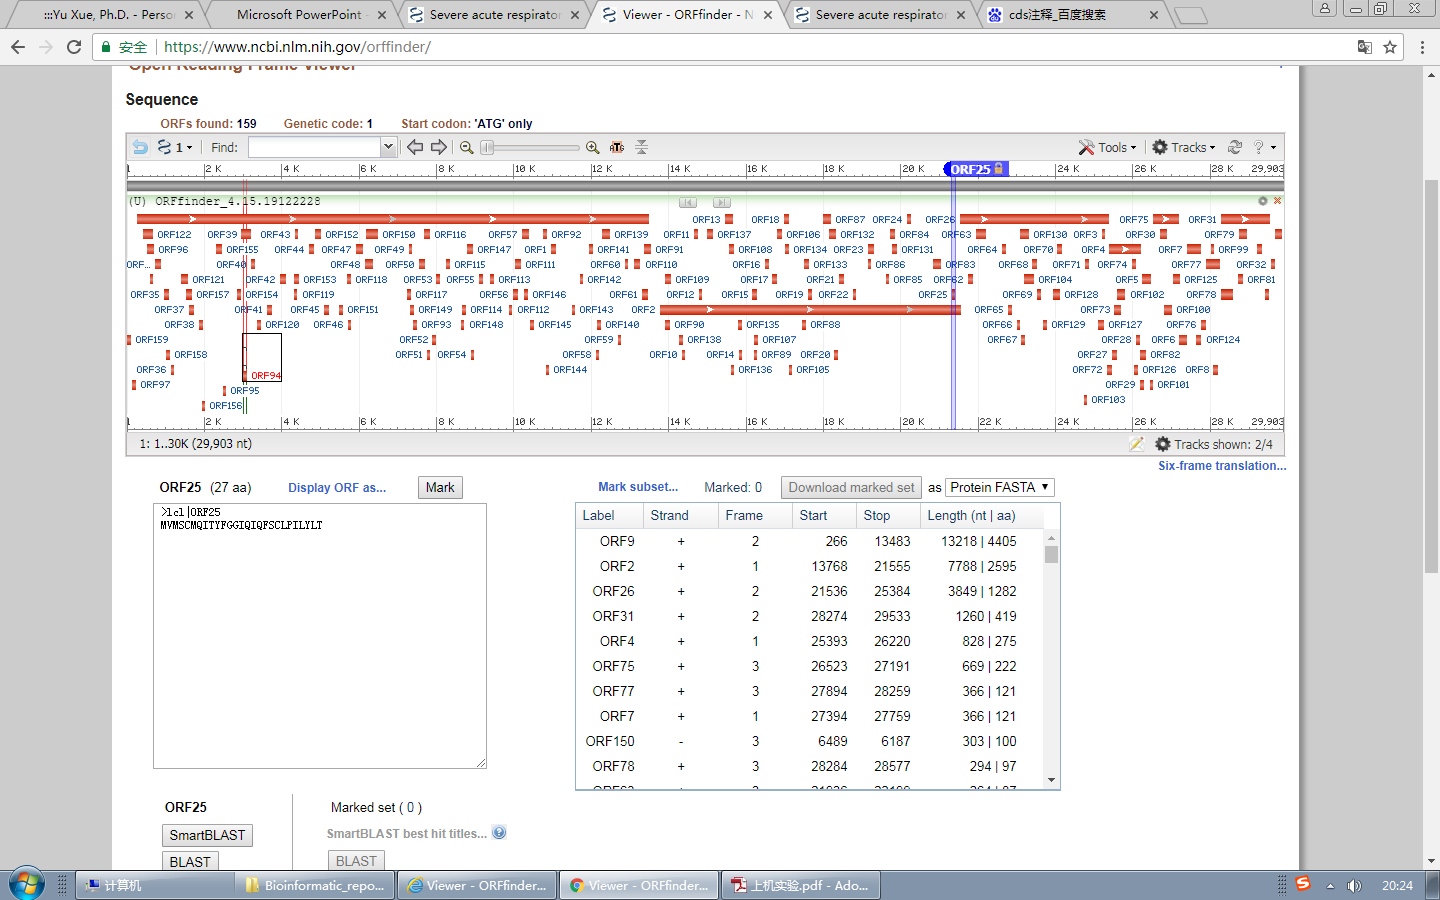
\includegraphics[width=1\textwidth]{./material/practice1/ORF.PNG}
    \caption{ORF\_prediction.PNG}
  \end{figure}
  \subsection{5.发现与SARS-CoV-2同源的冠状病毒}

  \subsection{6.插入片段分析}

	\section{序列分析}
	\subsection{1.INS1378与pShuttle-SN载体的相似性}

	\subsection{2.SARS-CoV-2的蛋白质序列}

	\subsection{3.等电点与分子量分析}
	\begin{table}[H]
  \begin{center}
    \caption{编码蛋白等电点与分子量}
    \begin{tabular}{l|c|r} % <-- Alignments: 1st column left, 2nd middle and 3rd right, with vertical lines in between
      \textbf{序号} & \textbf{等电点pI} & \textbf{分子量Mw}\\
      \hline
			  CDS\_1 & 6.32 & 794057.79\\
        CDS\_2 & 6.04 & 489988.91\\
        CDS\_3 & 6.24 & 141178.47\\
        CDS\_4 & 5.55 & 31122.94\\
        CDS\_5 & 8.57 & 8365.04\\
        CDS\_6 & 9.51 & 25146.62\\
        CDS\_7 & 4.60 & 7272.54\\
  	    CDS\_8 & 8.23 & 13744.17\\
  	    CDS\_9 & 4.17 & 5180.27\\
  	    CDS\_10 & 5.42 & 13831.01\\
  	    CDS\_11 & 10.07 & 45625.70\\
  	    CDS\_12 & 7.93 & 4449.23\\
    \end{tabular}
  \end{center}
\end{table}
	\subsection{4.功能结构域分析}

	\subsection{5.细胞亚定位分析}

\end{document}
